\documentclass{beamer}
% Setup appearance:
\usetheme{Marburg} 

\usepackage{color} % It may be necessary to set PCTeX or whatever program you are using to output a .pdf instead of a .dvi file in order to see color on your screen.
\usepackage{graphicx} 

\usepackage[spanish]{babel}
\usepackage[latin1]{inputenc}
\usepackage{amsmath}
\usepackage{mathtools}
\usepackage{calrsfs}
\usepackage{cases}
\usepackage{hyperref}

\usepackage{tikz}
\usetikzlibrary{arrows}
\tikzstyle{block}=[draw opacity=0.7,line width=1.4cm]


% Author, Title, etc.

\title[] 
{%
  Programaci�n de la EDU-CIAA en lenguaje C (\textit{sin RTOS})\\ 
 %5ta ESE - Horco Molle 2015 %
}
	
\author[]
{
Bioing.~Juan~Manuel Reta \\ Mgt Eduardo Filomena~\
}

%\insertshortdate
\date[2015]
{}


% The main document

\begin{document}

\begin{frame}
% \begin{center}

%\end{center}
  \titlepage
\begin{center}
  
	
\includegraphics[height=1cm]{Imagenes/logo_ruse}
\hspace{1cm}
	
\includegraphics[height=1cm]{Imagenes/acse}
\end{center}

\end{frame}

\section{Presentaci�n}

\subsection{Objetivos}

\begin{frame}{Objetivos del Curso}
\begin{itemize}
\item Analizar las principales caracter�sticas de la arquitectura de los microcontroladores ARM Cortex M4 en general y del LPC4337 en particular.
\item Estudiar el hardware de la EDU-CIAA-NXP y de la CIAA-NXP.
\item Presentar herramientas de gesti�n de repositorio.
\item Comprender los pasos de instalaci�n del IDE de la CIAA.
\item Analizar en forma general el est�ndar POSIX y sus ventajas.
\item Presentar el concepto de capa de abstracci�n de hardware (HAL) y ejercitar con la biblioteca LPCOpen.

\end{itemize}
\begin{flushright}
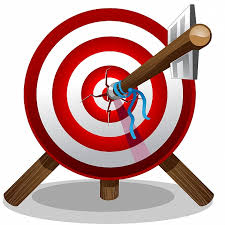
\includegraphics[height=2cm]{Imagenes/objetivo_rojo}
\end{flushright}

\end{frame}
\section{Historia}


\begin{frame}{Sistemas Embebidos}

\begin{columns}
\column{.6\textwidth}

 Eran los 60 y los laboratorios AT\&T Bell junto al MIT trabajaban en un sistema operativo experimental: Multics (Multiplexed Information and Computing Service), dise�ado para funcionar en un GE-645, un potente ordenador de aquella �poca. Ken Thompson y Dennis Ritchie son los responsables del proyecto.
\column{.4\textwidth}

\begin{figure}
	\centering
		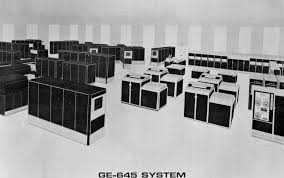
\includegraphics[height=2.5cm]{./Imagenes/GE-645}
	\label{fig:unix}
\end{figure}
\end{columns}
\vspace{.5cm}

\begin{itemize}
\item Multics no funcion� como se esperaba.
\item Ken Thompson y Dennis Ritchie, comenzaron a trabajar en un juego sobre la GE-645.
\item Al querer portar el \textit{Space Travel} a una PDP-7 teminaron desarrollando UNICS.
\item AT\&T Bell decidi� subvencionar el desarrollo incorporando programadores, entre ellos a Brian Kernighan. UNICS pasa a llamarse UNIX.
\end{itemize} 

%\end{block}

\end{frame}

\section{Sistemas Embebidos}

\begin{frame}{Sistemas Embebidos}

\begin{figure}
	\centering
		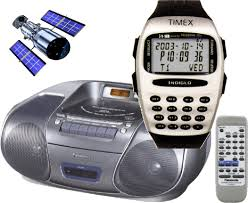
\includegraphics[height=4cm]{./Imagenes/embedded_system0}
	\label{fig:sis_embed}
\end{figure}

\begin{figure}
	\centering
		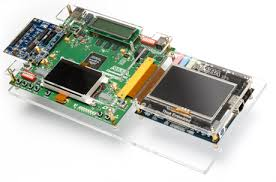
\includegraphics[height=3cm]{./Imagenes/embedded_system3}
	\label{fig:sis_embed2}
\end{figure}

\end{frame}



\begin{frame}

\begin{figure}
	\centering
		
\includegraphics[height=2cm]{./Imagenes/embedded_system1}
	\label{fig:sis_embed3}
\end{figure}

\begin{block}{Definici�n}
Un sistema embebido es un sistema electr�nico contenido -\textit{embebido}- dentro de un equipo completo que incluye otras partes (mec�nicas, electromec�nicas, etc.)
\begin{flushright}
{\tiny \textbf{\textit{JM. Cruz}}}
\end{flushright}
\end{block}

\end{frame}


\begin{frame}{Sistemas Embebidos}

En buena parte de las aplicaciones reales como cerebro de un sistema embebido se recurre a un microcontrolador.\\
\vspace{0.5cm}
Requisitos de Dise�o:\\
\begin{itemize}
\item Tama�o reducido, bajo consumo. 
\item Costo competitivo.
\item Eficiencia, confiabilidad y \textit{re-usabilidad}.
\item Determinismo y tiempo de respuesta �ptimo para la aplicaci�n.
\item Funcionalidades escalables.
\end{itemize}

\begin{figure}
	\flushright
		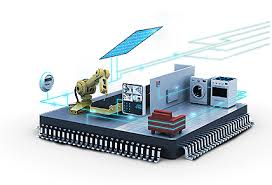
\includegraphics[height=2.5cm]{./Imagenes/micro_embedd1}
	\label{fig:micro_embedd}
\end{figure}

\end{frame}


\begin{frame}{Sistemas Embebidos}

\begin{columns}			
\column{.65\textwidth}
Hist�ricamente sea cual fuese la funci�n espec�fica del sistema embebido se ha requerido contar con:\\


\column{.30\textwidth}
\begin{figure}
	\flushright
		
\includegraphics[height=2cm]{./Imagenes/embedd}
	\label{fig:embedd}
\end{figure}

\end{columns}

\begin{itemize}
\item Las conectividades en uso corriente (USB, Ethernet, Wifi, Bluetooth, Zigbee, etc.)

\item Las interfaces de usuario en uso corriente (display LED, touch screen, multimedia, etc.)

\end{itemize}



\vspace{0.5cm}
�stos requerimientos (en permanente evoluci�n) obligan a contar con \textbf{plataformas} de rendimiento y \textbf{recursos en crecimiento} que permitan atender el incremento del procesamiento necesario para soportar nuevos perif�ricos con capacidad de atender las nuevas conectividades e interfaces de usuario requeridas por el mercado (usuarios)
\begin{flushright}
\textit{\textbf{{\tiny JM Cruz}}}
\end{flushright}

\end{frame}

\begin{frame}{El Paradigma}

\begin{figure}
	\centering
		
\includegraphics[height=3cm]{./Imagenes/hyS}
	\label{fig:hys}
\end{figure}

\begin{columns}			
\column{.65\textwidth}
\begin{itemize}
\item Pr�cticas de \textbf{Ingenier�a de Software} que sirvan para organizar el \textbf{ciclo de vida de un proyecto/producto} y mejorar la eficiencia del trabajo en equipo

\item T�cnicas de modelado en el desarrollo de sistemas embebidos.(Diagramas de Estado, de Actividad,UML)

\end{itemize}


\column{.40\textwidth}
\begin{figure}
	\flushright
		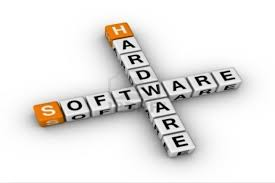
\includegraphics[height=2.7cm]{./Imagenes/hard_soft}
	\label{fig:hard_soft}
\end{figure}
\end{columns}
\end{frame}

\subsection{Software Embebido}
\begin{frame}
\begin{itemize}
\item \textbf{Funcionalidad} - �Qu� funcione bien!
\item \textbf{Confiable} -  Que funcione bien siempre
\item \textbf{Testeable} - Que resulte sencillo vericicar si funciona bien.
\item \textbf{Portable} - que pueda compilarse y correr en diferentes plataformas.
\item \textbf{Reusabilidad} - Que pueda se reutilizado para diferentes aplicaciones.
\item \textbf{Simple} - Sencillo de interpretar y mantener.
\end{itemize}

\begin{figure}
	\flushright
		
\includegraphics[height=2.7cm]{./Imagenes/good_soft}
	\label{fig:god_soft}
\end{figure}
\end{frame}

\begin{frame}

\begin{figure}
	\centering
		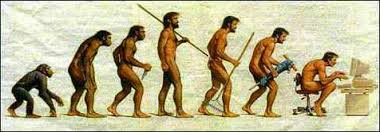
\includegraphics[height=2cm]{./Imagenes/evolution}
	\label{fig:evolution}
\end{figure}

\begin{figure}
	\centering
		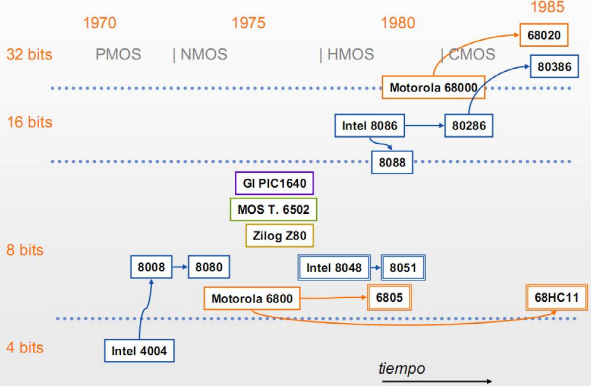
\includegraphics[height=6cm]{./Imagenes/evolucion_temporal}
	\label{fig:evol_micro}
\end{figure}

\end{frame}

\begin{frame}

\begin{figure}
	\centering
		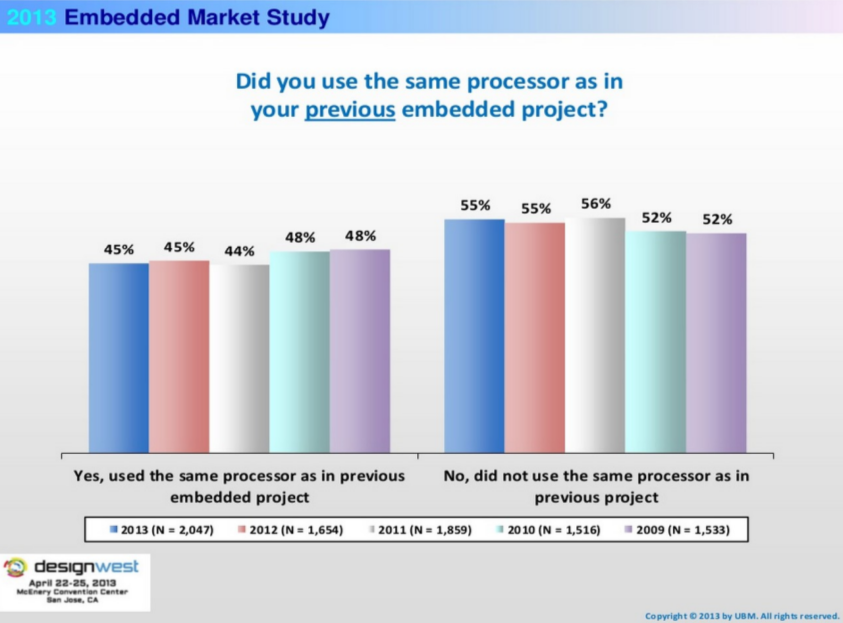
\includegraphics[height=5.5cm]{./Imagenes/uso_micros}
	\label{fig:arquitectura}
\end{figure}

\end{frame}

\begin{frame}{Datasheets}

\begin{figure}
	\centering
		
\includegraphics[height=3.5cm]{./Imagenes/manuals}
	\label{fig:manual}
\end{figure}

\end{frame}

\section{Hardware Abstraction Layer}

\begin{frame}

\begin{block}{Hardware Abastraction Layer}
Es la parte de software que se relaciona directamente con el hardware. Su funci�n es proveer una interfaz entre los recursos del hardware y la aplicaci�n o el sistema operativo. 
\end{block}

\begin{figure}
	\centering
		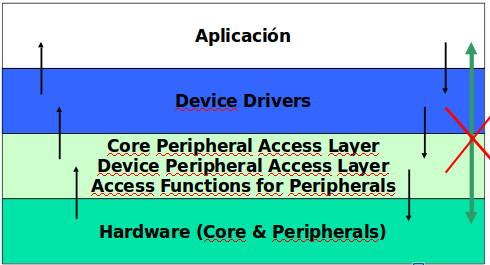
\includegraphics[height=4cm]{./Imagenes/hal}
	\label{fig:hal1}
\end{figure}
{\tiny \textbf{Fig: Ing. Juan Manuel Cruz}}
\end{frame}

\begin{frame}

\begin{figure}
	\centering
		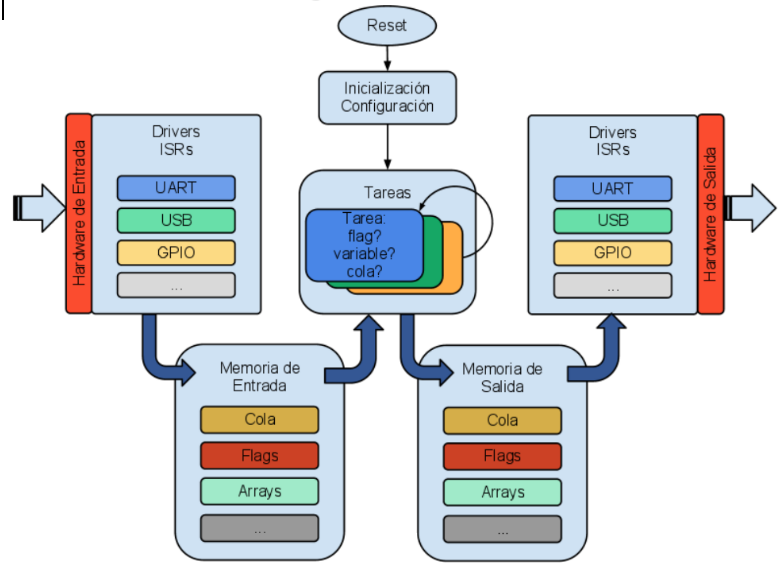
\includegraphics[height=5cm]{./Imagenes/estructura_soft}
	\label{fig:estructura_soft}
\end{figure}
\begin{flushright}
{\tiny \textbf{Fig: Ing. Juan Manuel Cruz}}
\end{flushright}

\end{frame}

\section{LPCOpen}

\begin{frame}

\begin{figure}
	\centering
		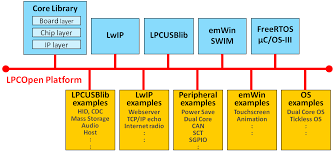
\includegraphics[height=4cm]{./Imagenes/lpcopen}
	\label{fig:lpcopen}
\end{figure}


\end{frame}


\end{document}
